\section{Modelliersprache}
Zur Beschreibung wurde, entgegen der in dem Projekt genannten Sprache, MyHDL\footnote{\url{http://myhdl.org}} genutzt. Es wurde uns von einem Kommilitonen nahe gelegt, \textit{nicht} VHDL zu nutzen, da es einen Großteil der Zeit in Anspruch nimmt, die Sprache zu lernen. Diese Zeit würde später fehlen, wenn man den Mikrocontroller implementieren möchte.
MyHDL ist ein Python-Modul, welches dazu genutzt wird Python als Hardwarebeschreibungssprache zu nutzen. Außerdem können damit auch Tests geschrieben werden, die zur Verifikation der Devices dient.
Ein Beispiel ist zu finden unter \autoref{HW:DFlipFop}.

\begin{figure}[h]
\small
\begin{pythoncode}
from myhdl import *
 
def dff(q, d, clk):
 
    @always(clk.posedge)
    def logic():
        q.next = d
 
    return logic
\end{pythoncode}
\caption{\label{HW:DFlipFop}D-FlipFlop}
\end{figure}

In Zeile drei werden sämtliche Ports der Komponente deklariert. Dabei werden -- im Gegensatz zu VHDL -- keine Spezifikationen wie input/output oder Bitlänge definiert. Diese werden laut Konvention nur in dem Kommentar der ``Funktion'' definiert.\\
Der Dekorator\footnote{\url{https://wiki.python.org/moin/PythonDecorators}} in Zeile 5 wird benutzt, um zu spezifizieren, wann die dekorierte Funktion ausgeführt werden soll. In diesem Fall besagt der Dekorator, dass bei einer steigenden Flanke des clk-Ports die Funktion ausgeführt werden soll.\\
Die eigentliche Logik der Komponente befindet sich in Zeile 7. Hier wird gesagt, dass im nächsten Augenblick der Wert von \textit{q d} sein soll.
In Zeile 9 wird die dekorierte Funktion zurückgegeben, d.h. sie wird in der Simulation und Transformation berücksichtigt.\\
Gut zu sehen sind an diesem Beispiel die Vor- und Nachteile von Python als Hardwarebeschreibungssprache. Ein Nachteil ist, dass man die genaue Spezifikation eines Ports nicht direkt angeben kann, z.B. deren Bitweite oder Typ. Dies kann zu Fehlern führen und zu viel Frust. MyHDL entscheidet die Eigenschaften durch statische Analyse des Quellcodes.\\
Vorteile hingegen sind der große Umfang der Python-Bibliotheken, die man sehr gut zum Testen der Komponenten nutzen kann, z.B. reguläre Ausdrücke, Listen oder Hashmap, sowie die einfache Erlernbarkeit und viele Syntaktische Feinheiten.\\

\section{Design}
\begin{figure}
\vspace{-4em}
\centering
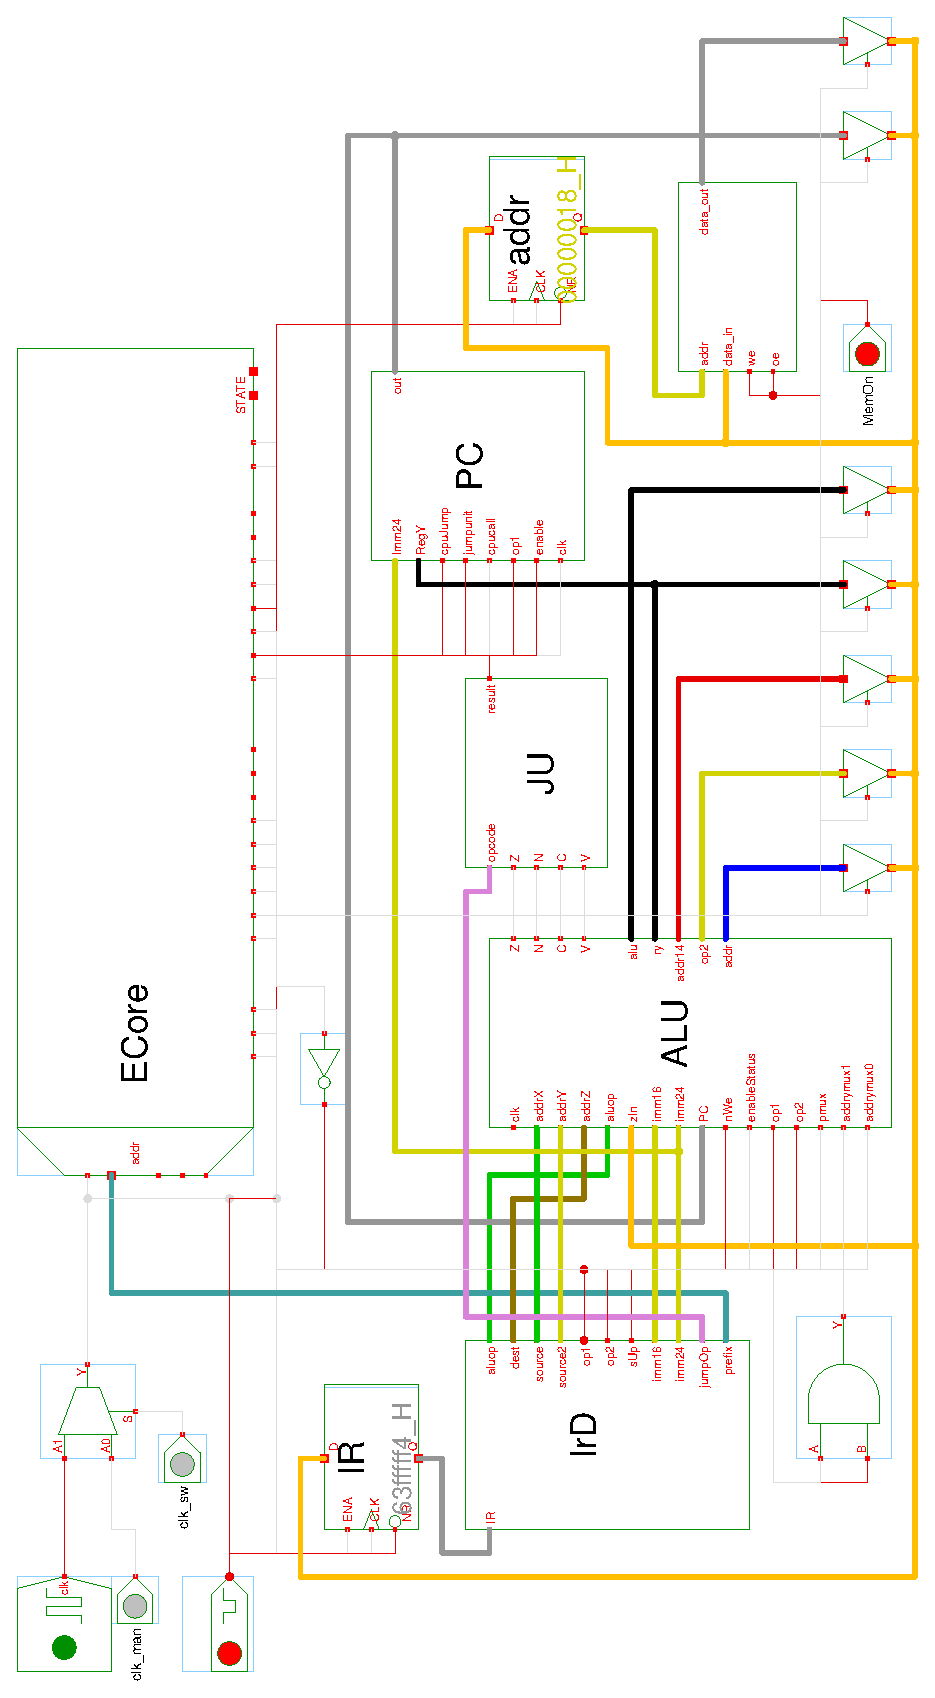
\includegraphics[width=.8\textwidth]{images/overview.eps}
\caption{\label{HW:Overview}Übersicht des MK}
\end{figure}
Das Design der Mikrocontrollers ist sehr stark am D-Core\footnote{\url{http://tams-www.informatik.uni-hamburg.de/applets/hades/webdemos/60-dcore/t3/processor.html}} orientiert, mit einem zentralen Bus, einem Steuerwerk, einer Abstraktion für den Speicher, sowie Elementen, die mit Hilfe des Busses miteinander kommunizieren. Wie man in der \autoref{HW:Overview} sehr gut sehen kann, ist die Verbindung zwischen den einzelnen Komponenten auf ein Minimum reduziert. Einzige Ausnahme bildet hierbei der Instruction-Decoder. Auf die einzelnen Komponenten wird in den Folgenden Abschnitten noch genauer eingegangen.\\
Die Entscheidung zu dieser Anordnung kam aus der Überlegung heraus, dass wir uns an etwas Bestehendem orientieren wollten. Deswegen verfügt er über einen Bus und verschiedene TriState-Dioden, die von einer Zentralen Einheit angesteuert werden, in unserem Fall das Steuerwerk oder CPU genannt. Doch genau hier liegt auch das Problem, denn die CPU ist nicht in der Lage, aktiv Werte an Komponenten zu senden, sondern schaltet nur Leitungen an oder aus. Auf dieses Problem wird später in der ALU auch noch genauer eingegangen. So gibt es an einigen Stellen für bestimmte Probleme maßgeschneiderte Lösungen.\\
Ein dennoch großer Vorteil eines gemeinsamen Busses ist die einfache Erweiterbarkeit des Systems. So hatten wir am Anfang gar nicht mit einer RS232-Schnittstelle gerechnet, konnte diese später jedoch problemlos einfügen, indem sie am Bus lauscht/schreibt und von der CPU geschaltet wird.\\
Die eigentliche Beschreibung des Mikrocontrollers erfolgt letztendlich in Python und kann im beigelegten Projektordner eingesehen werden.

\subsection{Steuerwerk}
Unser Steuerwerk (CPU) ist eine State-Maschine (\autoref{HW:CPU-State}), die anhand eines Präfix in den nächsten Status gelangt. In einem Status ist genau festgehalten, zu welchem Zeitpunkt welche Steuerleitung (de-)aktiviert wird. Hier ist es möglich, Substates zu haben (realsiert mit Hilfe eines hochlaufen Counters), falls dieser Befehl mehr als einen Takt benötigt. Außerdem ist es möglich, auf eingehende Signale zu warten, wie dies bei den Speicheroperationen der Fall ist. 

\begin{figure}[h]
\centering
\includegraphics[width=.7\textwidth]{images/cpustates.eps}
\caption{\label{HW:CPU-State}Cpu}
\end{figure}

Im Durchschnitt benötigt unsere CPU 8 Zyklen zum vollständigen Abarbeiten eines Befehls -- inklusive Laden und Warten. Dies ist allerdings nicht für alle Befehle so, denn z.B. benötigt man für eine Addition nur 5 Zyklen, wobei 4 für das Laden des Befehls verwendet werden. Platz für Optimierungen ist hier noch gegeben, z.B. könnte man die Speichereinheit auf der fallendenden Flanke operieren lassen. Auch haben wir keinerlei Mechanismen, die ein Pipelining ermöglichen oder s.g. \emph{Out-of-order Execution}, weil uns dies viel zu komplex und fehleranfällig erschien.

\subsection{Instruction Decoder}
Der Instruction Decoder (IrD) hat die Aufgabe, ein 32-Bit langes Wort in seine Einzelteile zu zerlegen und den einzelnen Komponenten zur Verfügung zu stellen. Dies soll nicht im Takt geschehen, sondern direkt. Die aktuelle Implementation ist in der \autoref{HW:IRD} zu sehen.\\
\begin{figure}[!ht]
\centering
\hspace{-5em}
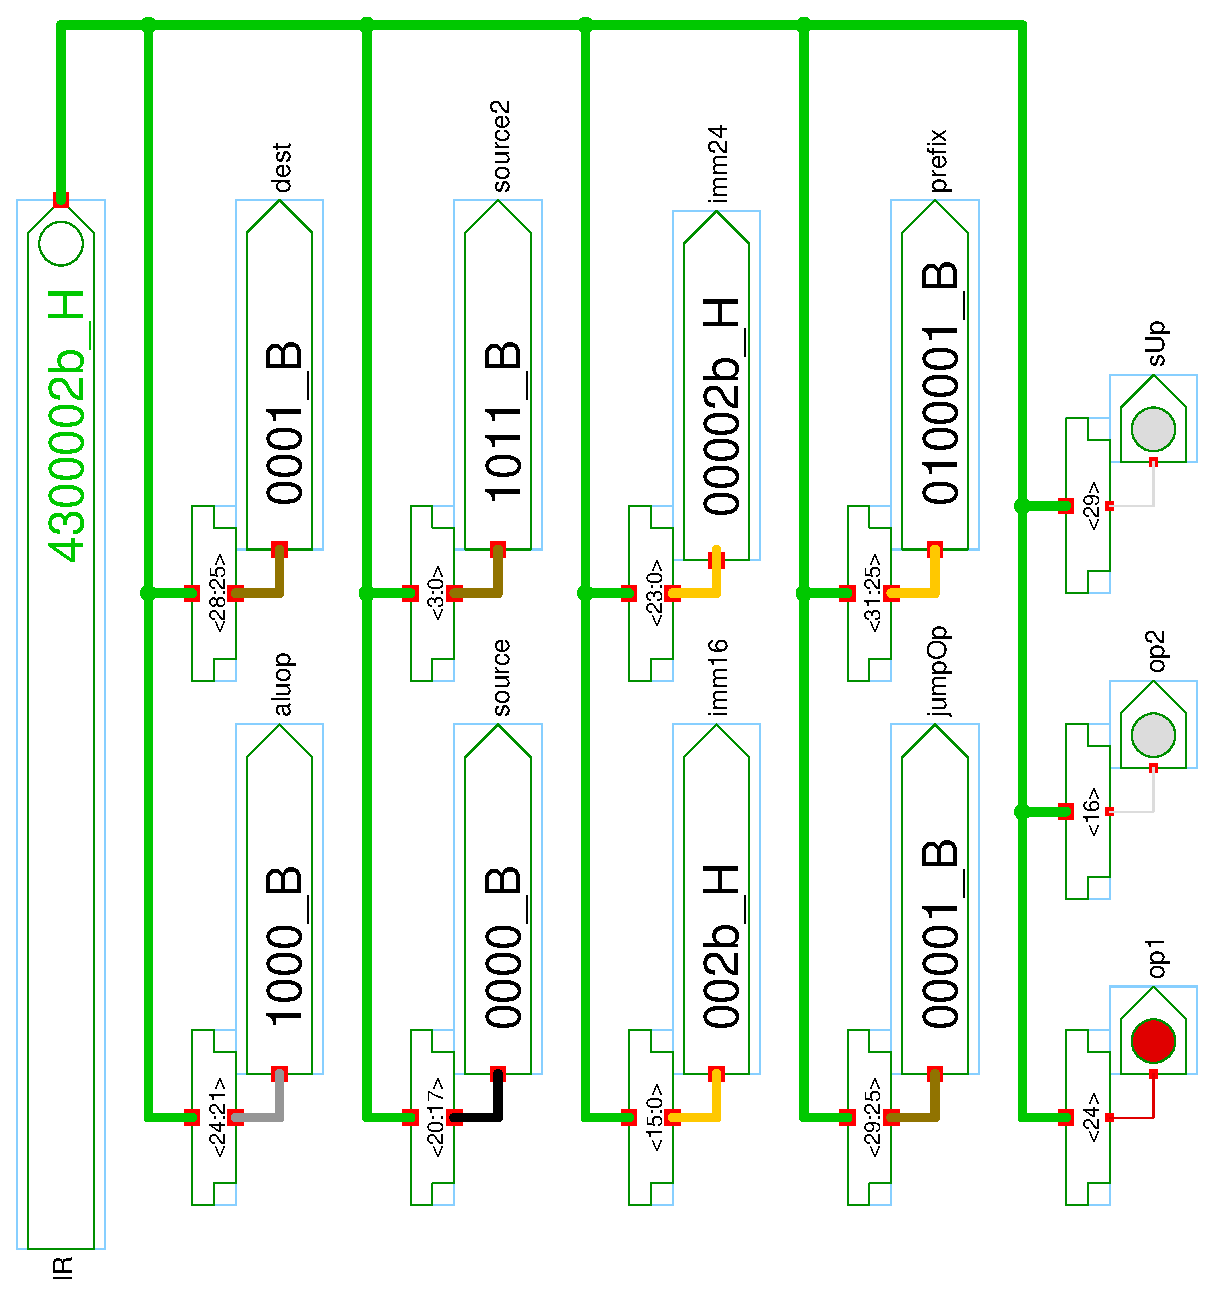
\includegraphics[width=1\textwidth,angle=270]{images/ir.eps}
\caption{\label{HW:IRD}Instruction Decoder}
\end{figure}%
Der IrD stellt 8 Werte und 3 Flags bereit.

\begin{itemize}
  \item aluop -- Der Op-code für die ALU
  \item dest --  Die Zieladresse für die Registerbank (Z)
  \item source -- Die erste Quelladresse für die Registerbank (X)
  \item source2 -- Die zweite Quelladresse für die Registerbank (Y)
  \item imm16 -- Ein 16-Bit breiter Immediate-Wert für Berechnungen
  \item imm24 -- Ein 24-Bit breiter Immediate-Wert für Berechnungen
  \item jumpop -- Der Op-code für die Sprungeinheit.
  \item prefix -- Das Instruktionsprefix für die CPU
\end{itemize}
Mit Hilfe der einzelnen Werte und Flags ist es nun möglich, einen Befehl gemäß unserer Befehlsstruktur auszuführen. Das Werte nicht immer sinnig sein müssen -- ein Sprungbefehl kann ein unsinniger Aluop sein -- ist für die Hardware nicht weiter schlimm, denn die Berchnung wird zwar ausgeführt, jedoch ihr Ergebnis nie auf den Bus schreiben, weil die CPU dies unterbindet.
\subsection{Adress, Arithmetisch und Logische Einheit}
Die Adress, Arithmetisch und Logische Einheit (kurz ALU) bildet ein Kernstück des Mikrocontrollers. Sie besteht aus mehreren Teilkomponenten die hier genauer erklärt werden.
\subsubsection{Registerbank}
\begin{figure}[!ht]
\centering
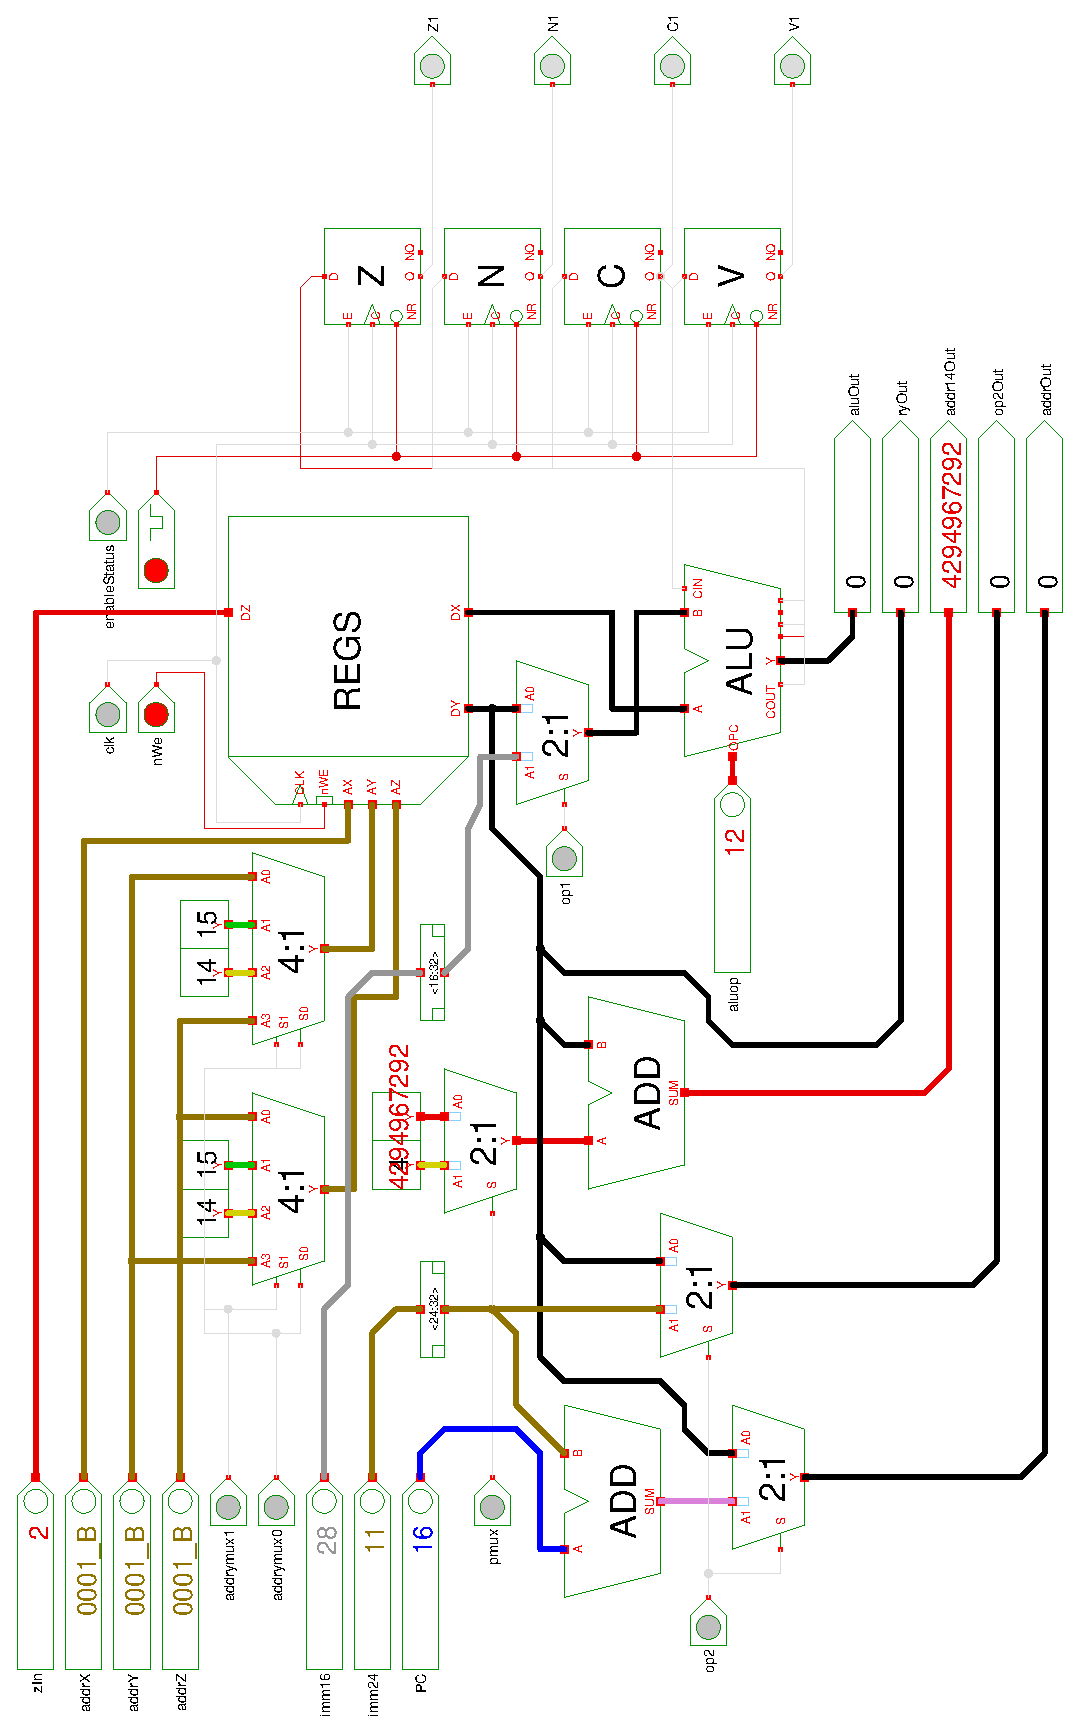
\includegraphics[width=.8\textwidth]{images/alu.eps}
\caption{\label{HW:ALU}Adress, Arithmetisch und Logische Einheit}
\end{figure}
Die ALU dient in unserem Mikrocontroller nicht allein zur Berechnung von Ergebnissen, sondern sie ist ein Sammelbegriff für alle Arten von mathematischen Operationen, wie z.B. Adress- oder Stackoffsetberechnung.\\
Die Registerbank hat 16 Slots, wobei einigen Plätzen besondere Eigenschaften und Bedeutungen zugewiesen wird. Dies hat nichts mit der ABI der Programme zu tun, sondern ist in der Hardware festgelegt und verdrahtet.
\begin{itemize}
  \item[0 --] Diese Adresse ist immer 0 und kann sowohl gelesen als auch beschrieben werden. Der Wert ändert sich nie.
  \item[14 --] Die Addresse ist der Stackpointer. Wann immer eine Push/Pop Operation ausgeführt wird, wird das 14te Register mit Hilfe der Hardware angepasst.
  \item[15 --] Die Rücksprungadresse. Mit Hilfe des Call-Befehl wird der aktuelle Programmcounter in das Register 15 abgelegt.
\end{itemize}
Um von der CPU aus die Adresse 14 bzw. 15 setzen zu können, sind zwei Multiplexer vor der Registerbank angebracht und steuerbar. Im Normalfall werden die Werte addrY/Z direkt an die Registerbank angelegt und die Werte ausgegeben. Wenn eine Stackoperation (\emph{Push/Pop}) ausgeführt wird, wird die Steuerleitung \textit{addrymux1} gesetzt und eine konstante 14 an die Adressleitungen Y und Z gelegt. Wenn ein \emph{Call} oder \emph{Ret} ausgeführt wird, wird der Wert aus der Adresse 15 benötigt und die Leitung \textit{addrymux0} gesetzt. Für einige Befehle befindet sich die Y oder Z Adresse an der \glqq falschen\grqq \ Stelle und muss getauscht werden. Dies wird erreicht, indem beide Steuerleitungen \textit{addrymux0} und \textit{addrymux1} gesetzt werden.

\subsubsection{Recheneinheit}
Die Recheneinheit (ALU) kann 16 Befehle verarbeiten (eine Übersicht ist zu sehen in \autoref{AP:ISA}) und verarbeitet hierbei zwei 32-Bit Werte plus ein Carry in. Das entsprechende Ergebnis ist ebenfalls 32-Bit breit. Außerdem werden s.g. Statusflags berechnet und bei Bedarf (siehe ISA) gesetzt. Diese werden für die Sprungheinheit benötigt. Der erste Eingang ist immer ein Wert aus der Registerbank (Adresse X), der zweite ist abhängig vom Befehl. Entweder ebenfalls aus der Registerbank (Addresse Y) oder ein 16-Bit Immediate, der auf 32-Bit \glqq Vorzeichenerweitert\grqq \footnote{D.h. das Vorzeichen des kleinen Wertes wird auf den großen Wert übertragen} und so verrechnet wird.

\subsubsection{Adressberechnungen}
Die ALU übernimmt außerdem viele Adressberechnungen, z.B. für Sprünge, Funktionsaufrufe oder Stackoperationen.
Sprünge werden entweder direkt ausgeführt (Registersprung) oder relativ zum aktuellen Programmcounter (Immediate24+Offset). Deshalb wird mit Hilfe eines Multiplexers und einer Flag aus dem IrD entschieden, welche Adressierungsart erfolgen soll.
Für die Stackoperationen wird direkt die nachfolgende Adresse berechnet, entweder +4 (\emph{Pop}) oder -4 (\emph{Push}). Die Subtraktion wird mit Hilfe der Addition des Zweierkomplements durchgeführt.
Auch erlaubt die ALU es, den Op2 direkt auf den Bus zu schreiben. Hierfür bedient man sich lediglich eines einfachen Multiplexers.

\subsection{Jumpunit}
\begin{figure}[!ht]
\centering
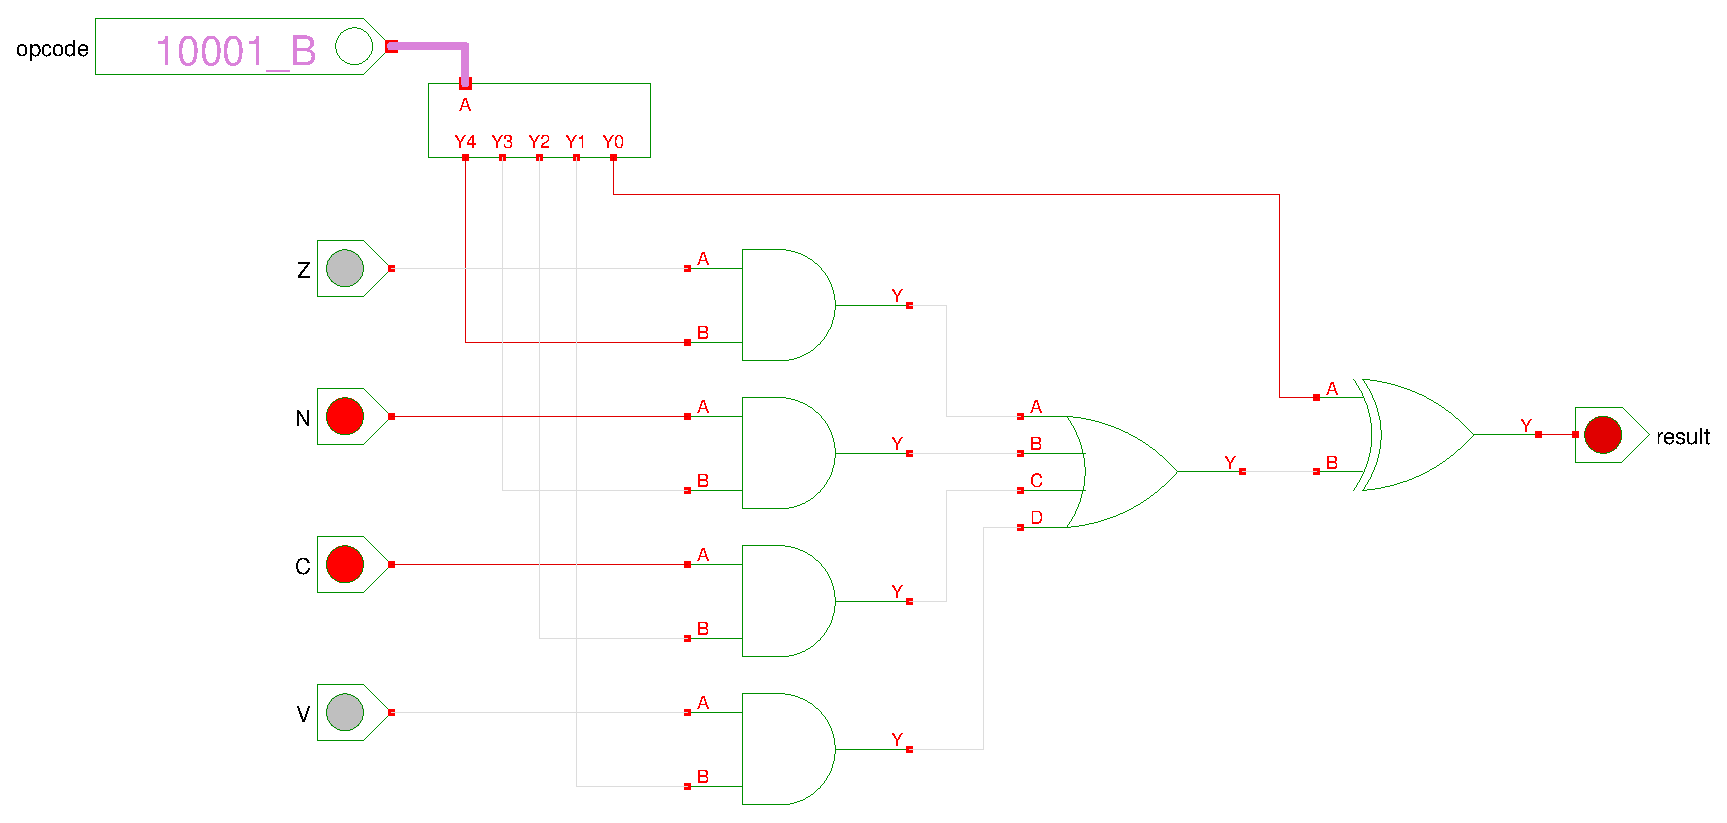
\includegraphics[width=1\textwidth]{images/ju.eps}
\caption{\label{HW:JU}Sprung-Einheit}
\end{figure}
Die Sprungeinheit entscheidet anhand der Statusflags und des Jumpopcodes aus dem IrD, ob ein Sprung erfolgen soll. Der Jumpcode besteht aus 5 Bit, wobei die obersten 4 Bit entscheiden, ob das entsprechende Statusbit berücksichtigt werden soll und das unterste Bit die Entscheidung invertiert. Die Bits 4 bis 1 stehen für:
\begin{enumerate}
 \item[4] -- Zero-Flag
 \item[3] -- Negative-Flag
 \item[2] -- Carry-Flag
 \item[1] -- Overflow-Flag
\end{enumerate}
Ob letztendlich ein Sprung erfolgen soll, wird im Programmcounter entschieden.
\subsection{Programmcounter}
\begin{figure}[!ht]
\centering
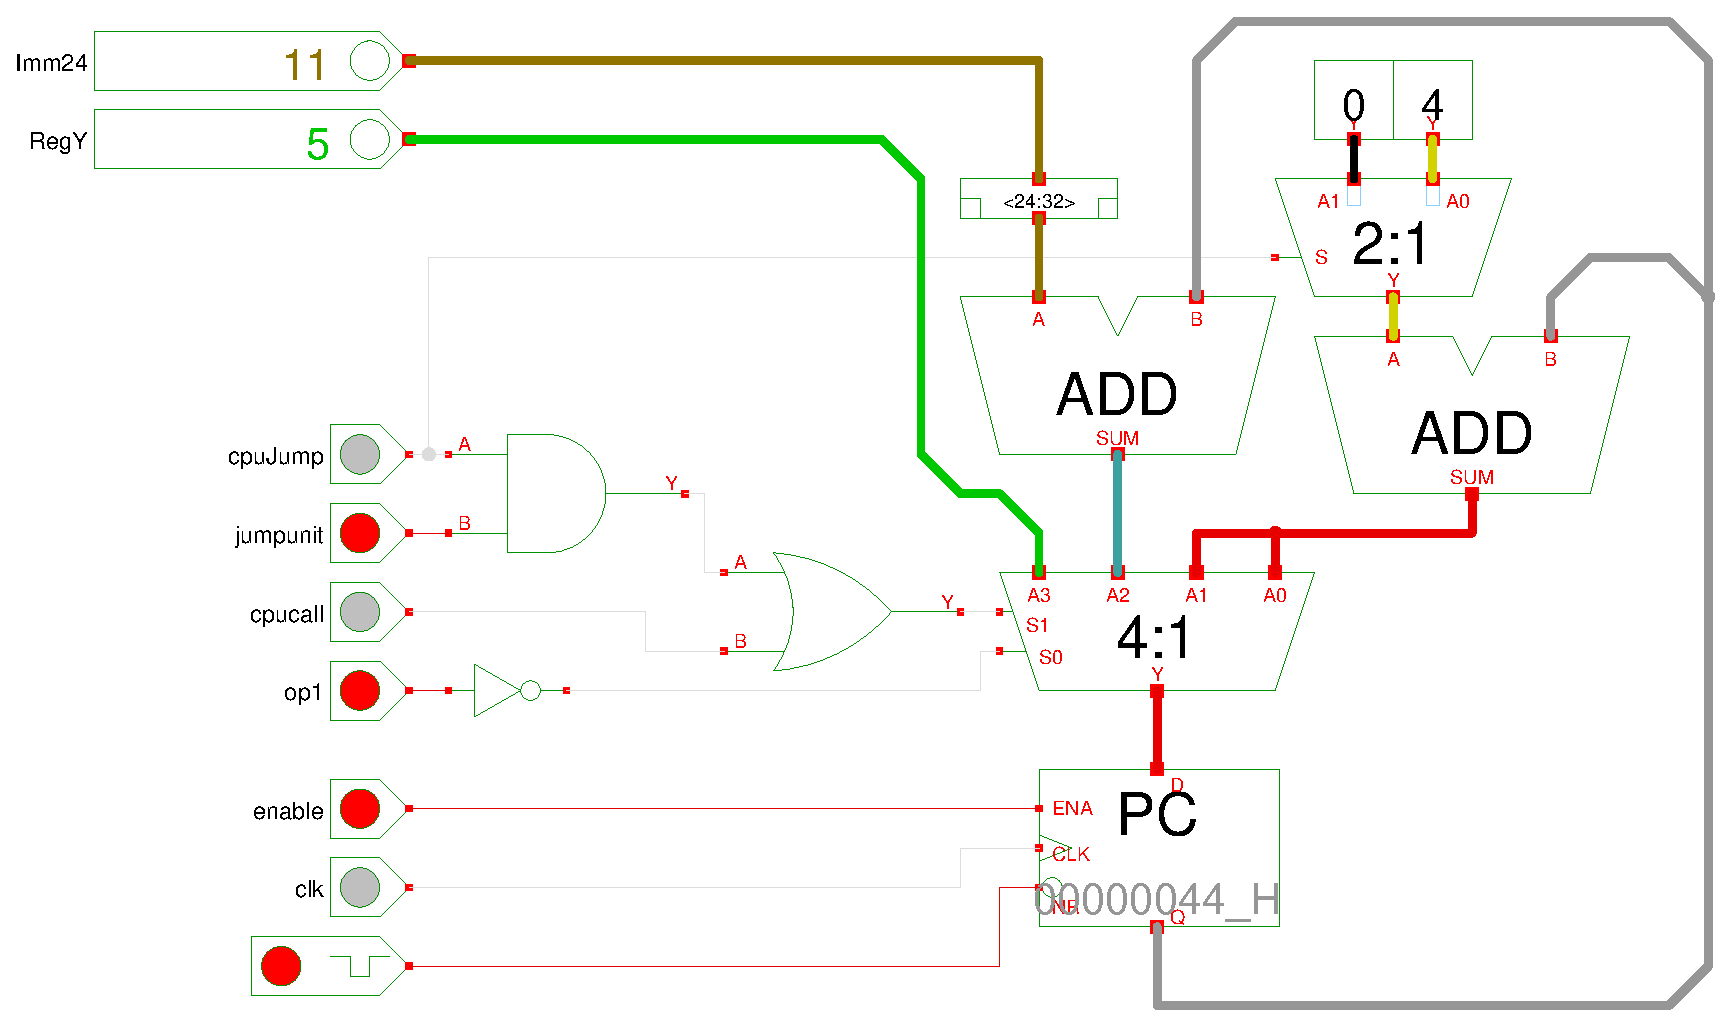
\includegraphics[width=1\textwidth]{images/pc.eps}
\caption{\label{HW:PC}Programmcounter}
\end{figure}
Der Programmcounter hält fest, an welcher Speicheradresse wir uns im Code befinden. Außerdem hat er die Aufgabe, die Folgeadresse anhand von Flags und Eingaben zu berechnen.
Der Standard ist, dass der Programmcounter um 4 erhöht wird. Wir haben uns für eine wortweise Adressierung entschieden, da dies das Verhalten von gängigen Prozessoren ist und wir so auch auf halbe Befehle springen können. Dies ist zwar bis jetzt nicht nötig, aber kann sie als sinnvoll herausstellen.\\
Der PC erhöht seinen Wert nur, wenn von der CPU ein entsprechendes Signal kommt. Auch kann die CPU einen Sprung veranlassen -- direkt, d.h. ohne die Entscheidung der JumpUnit mit dem \emph{cpucall} Flag oder mit Hilfe der JumpUnit und dem \emph{cpujump} Flag. Wie schon in der ALU kann hier absolut (mit dem RegY-Wert aus der Registerbank) oder indirekt, d.h. $PC+Imm24$ gesprungen werden. Dabei ist zu beachten, dass auch hier die 24-Bit Sign-Extended werden müssen, da sonst keine negativen Sprünge möglich sind.

\section{Realisierung}
Da wir nicht VHDL nutzten sondern MyHDL, mussten wir uns erst einmal in das Framework einarbeiten. Dies gelang erstaunlich gut, denn es gibt ein paar gute Beispiele auf der Homepage. In der anfangs genutzten Version 0.8 waren jedoch ein paar Fehler enthalten. Da das Framework jedoch Opensource ist, konnten wir uns den Sourcecode direkt von bitbucket\footnote{\url{https://bitbucket.org/jandecaluwe/myhdl}} herunterladen. In dem Projekt nutzten wir eine modifizierte Version 0.9. Unsere Patches sind direkt in das Projekt eingeflossen und sind nun teil des Frameworks\footnote{Zur Zeit fehlt noch ein Commit}.\\
Da das Altera-Programm logischerweise keinen MyHDL Code annimmt, muss dieser erst konvertiert werden. Dabei gibt es zwei Möglichkeiten -- entweder VHDL oder Verilog. Wir haben uns für Verilog entschieden, da der Code verständlicher ist und auch weniger Nachbearbeitung bedarf. Man muss schlussendlich einen Wrapper für den generierten Code schreiben, damit die Pins zugeordnet und genutzt werden können. Anschließend kann die Altera-Software den Code verwerten und auf den FPGA bringen.
